\block{}{
	\begin{itemize}[leftmargin=1.5em]
		\item \textbf{Líderes de Crecimiento:} Juana Díaz, Carolina y Manatí encabezan la lista con tendencias positivas ($\approx 0.002$), sugiriendo una expansión en la eficiencia de uso de energía relativa a sus insumos de capital y trabajo.
		\item \textbf{Zonas de Declive:} Cidra, Aguada y Canóvanas muestran las tendencias más bajas ($\approx -0.003$), lo que podría indicar estancamiento industrial o procesos de deseconomía de escala en el periodo 2021-2024.
	\end{itemize}

	\begin{tikzfigure}[Estimacion de importaciones del sector 11]
		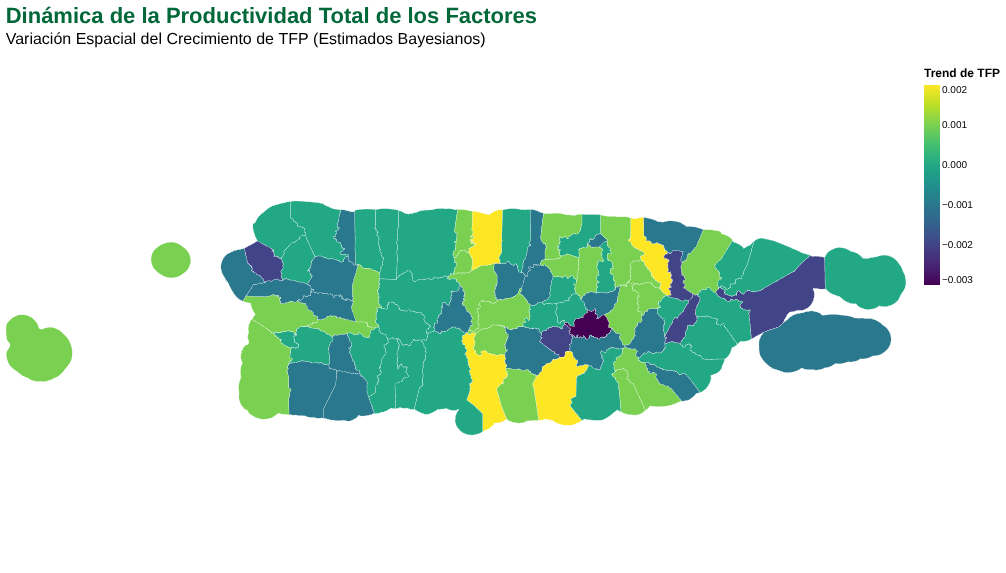
\includegraphics[width=1\linewidth]{assets/maps.png}
	\end{tikzfigure}
}


